\documentclass[12pt,a4paper]{article}
\usepackage{fontspec}
\setmainfont{Times New Roman}
\setsansfont{Arial}
\setmonofont{Courier New}
\usepackage[provide=*,english,romanian]{babel}
\usepackage{amsmath,amssymb,graphicx,geometry,setspace}
\usepackage{fancyhdr,caption,float,listings,xcolor,booktabs,longtable,array,calc}
\usepackage{subcaption,etoolbox,upquote}
\usepackage[unicode,hidelinks]{hyperref}
\geometry{top=2cm,bottom=2cm,left=2.5cm,right=2.5cm}
\setstretch{1.5}
\setlength{\parindent}{0pt}
\setlength{\parskip}{5pt}
\makeatletter
\renewcommand\section{\@startsection{section}{1}{0pt}{16pt}{7pt}{\normalfont\Large\bfseries}}
\renewcommand\subsection{\@startsection{subsection}{2}{0pt}{12pt}{5pt}{\normalfont\large\bfseries}}
\renewcommand\subsubsection{\@startsection{subsubsection}{3}{0pt}{9pt}{4pt}{\normalfont\normalsize\bfseries}}
\makeatother
\setcounter{secnumdepth}{-1}
\pagestyle{fancy}
\fancyhf{}
\rfoot{\thepage}
\renewcommand{\headrulewidth}{0pt}
\setlength{\headheight}{15pt}
\captionsetup{font=small,labelfont=bf,skip=6pt,justification=raggedright,singlelinecheck=false}
\captionsetup[figure]{position=above}
\lstset{language=C,basicstyle=\ttfamily\fontsize{9.5}{11.5}\selectfont,
  columns=fullflexible,showstringspaces=false,tabsize=2,numbersep=8pt,
  frame=single,rulecolor=\color{black!35},breaklines=true,keepspaces=true,
  xleftmargin=4pt,xrightmargin=4pt,aboveskip=8pt,belowskip=8pt}
\AtBeginEnvironment{lstlisting}{\singlespacing}
\AtBeginEnvironment{longtable}{\small\singlespacing}
\setlength{\emergencystretch}{3em}
\providecommand{\tightlist}{\setlength{\itemsep}{0pt}\setlength{\parskip}{0pt}}
\providecommand{\passthrough}[1]{#1}
\providecommand{\pandocbounded}[1]{#1}
\hypersetup{pdftitle={Sisteme de operare — Laborator 18},pdfauthor={Tacu Igor}}
\clubpenalty=10000
\widowpenalty=10000
\displaywidowpenalty=10000
\begin{document}
\begin{titlepage}
\thispagestyle{empty}
\begin{center}
\setstretch{1.18}

\includegraphics[width=0.23\textwidth]{scripts/report-style/utm-logo.png}\\[12pt]
\textbf{MINISTERUL EDUCAȚIEI ȘI CERCETĂRII}\\
\textbf{AL REPUBLICII MOLDOVA}\\[4pt]
\textbf{Universitatea Tehnică a Moldovei}\\
\textbf{Facultatea de Calculatoare, Informatică și Microelectronică}\\
\textbf{Departamentul Inginerie Software și Automatică}\\[36pt]
{\fontsize{22}{26}\selectfont\textbf{Raport}}\\[10pt]
Lucrare de laborator nr. 18\\[8pt]
\textbf{\large Sisteme de operare}\\[24pt]
\textbf{Tema:} Comutarea contextului firelor în spațiul utilizatorului xv6
\end{center}
\vfill
\begin{flushright}
\setstretch{1.25}
Realizat de:\\
stud. gr. FAF-242, Tacu Igor\\[24pt]
Verificat de:\\
Reițman Patricia
\end{flushright}
\vfill
\begin{center}\textbf{Chișinău – 2026 }\end{center}
\end{titlepage}

\setcounter{page}{1}
\section{Scopul lucrării}\label{scopul-lucrux103rii}

Implementarea unei comutări cooperative între fire user prin salvarea și
restaurarea registrelor și schimbarea stivei.

\section{Sarcina lucrării}\label{sarcina-lucrux103rii}

\begin{itemize}
\tightlist
\item
  Completarea contextului ra, sp și s0--s11 și inițializarea fiecărui
  fir.
\item
  Implementarea rutinei assembly și integrarea programului în Makefile.
\item
  Verificarea alternării celor trei fire până la 99 și explicarea
  rolului registrului ra.
\end{itemize}

\section{Considerații teoretice}\label{consideraux21bii-teoretice}

Un apel de funcție are registre păstrate de apelat și registre pe care
apelantul le poate considera modificate. O comutare cooperativă
păstrează ra, sp și registrele s, apoi ret continuă în contextul
selectat. Firele user partajează un proces și cedează explicit controlul
prin yield.

\section{Implementare. Rezultate
practice}\label{implementare.-rezultate-practice}

\subsection{Scope and execution
environment}\label{scope-and-execution-environment}

The supplied Lab 18 handout requests completion of
{\ttfamily\fontsize{10}{12}\selectfont user/uthread\allowbreak{}.c}, a
RISC-V assembly switch in
{\ttfamily\fontsize{10}{12}\selectfont user/uthread\allowbreak{}\_switch.S},
an explicit Makefile link rule, and the Observe answer in
{\ttfamily\fontsize{10}{12}\selectfont notes.txt}. All implementation
files are submitted in the canonical
{\ttfamily\fontsize{10}{12}\selectfont xv6/} tree. No kernel source was
changed for this laboratory. This is a completed version of the supplied
skeleton, adapted only with a check for exhausted thread slots and
explicit zeroing of newly created contexts.

The real tree was built and run on the Ubuntu server on 24 November 2026
using the RISC-V cross toolchain and QEMU with three virtual CPUs. The
isolated execution copy is
{\ttfamily\fontsize{10}{12}\selectfont /root/os-lab\allowbreak{}18/xv6}.
The existing Labs 4--13 programs remain registered. The xv6 tree comes
from MIT under its included license; the handout supplies the scheduler
structure and demonstration, while the context implementation and
validation were completed with coding assistance.

{\ttfamily\fontsize{10}{12}\selectfont evidence/bui\allowbreak{}ld.txt}
retains the real full-tree build. The build completed; the linker emits
the existing RWX LOAD-segment warnings for the kernel and small
{\ttfamily\fontsize{10}{12}\selectfont forktest} binary.
{\ttfamily\fontsize{10}{12}\selectfont evidence/exe\allowbreak{}cution.txt}
contains complete QEMU output for ten runs, and
{\ttfamily\fontsize{10}{12}\selectfont evidence/res\allowbreak{}ults.json}
records the checked counts and trace regression. The supplied native
Terminal captures show context layout, initial register values, the link
rule and the complete assembly switch. The native startup and
execution-final captures are also embedded below, completing the
four-image evidence set.
{\ttfamily\fontsize{10}{12}\selectfont CAPTURES.md} retains the live
reproduction commands; recorded text output below is distinguished from
native images.

\subsection{Part 1 --- Context layout and initial
execution}\label{part-1-context-layout-and-initial-execution}

The C context has fourteen eight-byte fields, in the same order used by
the assembly routine:

\par\noindent\begin{minipage}{\linewidth}

\begin{lstlisting}[language=C]
struct context {
  uint64 ra, sp;
  uint64 s0, s1, s2, s3, s4, s5, s6, s7, s8, s9, s10, s11;
};
\end{lstlisting}

\end{minipage}\par

{\def\LTcaptype{table} % do not increment counter
\begin{longtable}[]{@{}lrl@{}}
\toprule\noalign{}
Register & Offset & Role \\
\midrule\noalign{}
\endhead
\bottomrule\noalign{}
\endlastfoot
ra & 0 & Return continuation, or entry function for a new thread \\
sp & 8 & Current stack pointer \\
s0--s11 & 16--104 & Twelve callee-saved integer registers \\
\end{longtable}
}

Each thread has an 8,192-byte stack aligned to 16 bytes. The stack size
is itself a multiple of 16, so its initial top is aligned. Thread
creation finds a FREE slot, rejects exhaustion, clears its context, and
sets:

\par\noindent\begin{minipage}{\linewidth}

\begin{lstlisting}[language=C]
memset(&t->ctx, 0, sizeof(t->ctx));
t->ctx.ra = (uint64)func;
t->ctx.sp = (uint64)(t->stack + STACK_SIZE);
t->state = RUNNABLE;
\end{lstlisting}

\end{minipage}\par

On the first selection, the switch loads this synthetic context. Its
{\ttfamily\fontsize{10}{12}\selectfont ret} enters the function on that
thread's stack. On later selections, the same fields contain a real
suspended continuation and stack pointer.

The scheduling branch preserves the address of the old thread before
changing the global current pointer:

\par\noindent\begin{minipage}{\linewidth}

\begin{lstlisting}[language=C]
struct thread *old = current_thread;
next_thread->state = RUNNING;
current_thread = next_thread;
thread_switch(&old->ctx, &next_thread->ctx);
\end{lstlisting}

\end{minipage}\par

A yielding worker marks itself RUNNABLE; a finishing worker marks itself
FREE. The search starts after the current slot and wraps around,
selecting the next runnable context. The main context creates three
workers and frees its own slot before giving control to the scheduler.
Worker functions explicitly schedule again at their end; this small
exercise does not provide a general return trampoline or a join API.

\subsection{Assembly switch and build
integration}\label{assembly-switch-and-build-integration}

The complete switch mirrors the integer context shape of the existing
{\ttfamily\fontsize{10}{12}\selectfont kernel/swtch\allowbreak{}.S}, but
executes in user space:

\begin{lstlisting}
# Lab 18: offsets match struct context in user/uthread.c.
.text
.globl thread_switch
thread_switch:
        sd ra, 0(a0)
        sd sp, 8(a0)
        sd s0, 16(a0)
        sd s1, 24(a0)
        sd s2, 32(a0)
        sd s3, 40(a0)
        sd s4, 48(a0)
        sd s5, 56(a0)
        sd s6, 64(a0)
        sd s7, 72(a0)
        sd s8, 80(a0)
        sd s9, 88(a0)
        sd s10, 96(a0)
        sd s11, 104(a0)

        ld ra, 0(a1)
        ld sp, 8(a1)
        ld s0, 16(a1)
        ld s1, 24(a1)
        ld s2, 32(a1)
        ld s3, 40(a1)
        ld s4, 48(a1)
        ld s5, 56(a1)
        ld s6, 64(a1)
        ld s7, 72(a1)
        ld s8, 80(a1)
        ld s9, 88(a1)
        ld s10, 96(a1)
        ld s11, 104(a1)
        ret
\end{lstlisting}

The routine stores the old register set through
{\ttfamily\fontsize{10}{12}\selectfont a0}, restores the next set
through {\ttfamily\fontsize{10}{12}\selectfont a1}, then executes
{\ttfamily\fontsize{10}{12}\selectfont ret}. No system call,
address-space change or kernel scheduling operation is required for this
user-level switch. All workers share globals in one process while
retaining separate stacks and saved callee-saved registers.

The explicit link rule includes both C and assembly objects:

\par\noindent\begin{minipage}{\linewidth}

\begin{lstlisting}[language=make]
$U/_uthread: $U/uthread.o $U/uthread_switch.o $(ULIB) $U/user.ld
    $(LD) $(LDFLAGS) -T $U/user.ld -o $@ $U/uthread.o $U/uthread_switch.o $(ULIB)
    $(OBJDUMP) -S $@ > $U/uthread.asm
\end{lstlisting}

\end{minipage}\par

{\ttfamily\fontsize{10}{12}\selectfont \$U/\_uthread} is also registered
in UPROGS, so {\ttfamily\fontsize{10}{12}\selectfont make fs.img} places
it in the xv6 filesystem. The required changes are limited to two new
user source files and the Makefile.

\subsection{Native Terminal evidence --- context initialization and link
rule}\label{native-terminal-evidence-context-initialization-and-link-rule}

\par\medskip\noindent\begin{minipage}{\linewidth}\setstretch{1.0}
\captionof*{figure}{Figura 1. Native Terminal: context fields, aligned thread stack, initial ra and sp, and explicit uthread link rule}
\centering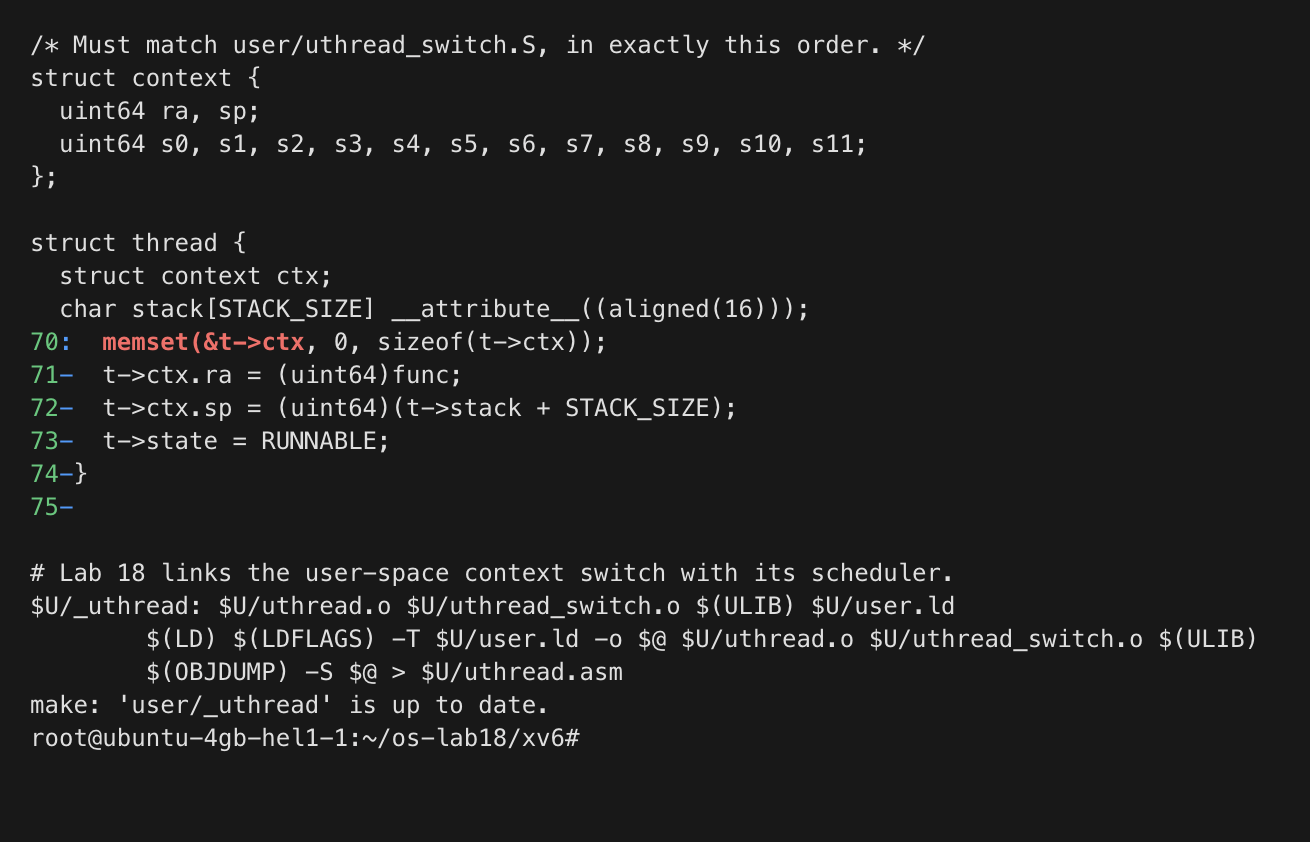
\includegraphics[width=\linewidth,height=0.67\textheight,keepaspectratio]{Lab18/evidence/screenshots/lab18-context-build-terminal.png}
\end{minipage}\par\medskip

The capture shows {\ttfamily\fontsize{10}{12}\selectfont ra},
{\ttfamily\fontsize{10}{12}\selectfont sp}, and
{\ttfamily\fontsize{10}{12}\selectfont s0–s11} in the required order,
followed by the thread context and 16-byte-aligned stack declaration.
Lines 70--73 clear the saved context, set
{\ttfamily\fontsize{10}{12}\selectfont ra} to the entry function, set
{\ttfamily\fontsize{10}{12}\selectfont sp} to the stack top, and mark
the slot RUNNABLE. The explicit Makefile rule links both
{\ttfamily\fontsize{10}{12}\selectfont uthread.o} and
{\ttfamily\fontsize{10}{12}\selectfont uthread\_swit\allowbreak{}ch.o}
with the user library and linker script.

The final {\ttfamily\fontsize{10}{12}\selectfont make} message is
{\ttfamily\fontsize{10}{12}\selectfont user/\_uthrea\allowbreak{}d is up to date}:
this invocation checks an existing executable rather than showing a
fresh compilation. The actual full build and subsequent QEMU runs are
retained separately in the evidence logs. This source capture
establishes initialization and integration; the assembly capture below
documents the register transfer, and the native execution-final capture
below shows the last rounds and worker termination.

\subsection{Native Terminal evidence --- complete assembly
switch}\label{native-terminal-evidence-complete-assembly-switch}

\par\medskip\noindent\begin{minipage}{\linewidth}\setstretch{1.0}
\captionof*{figure}{Figura 2. Native Terminal: fourteen register stores, fourteen matching loads and ret in uthread\_switch.S}
\centering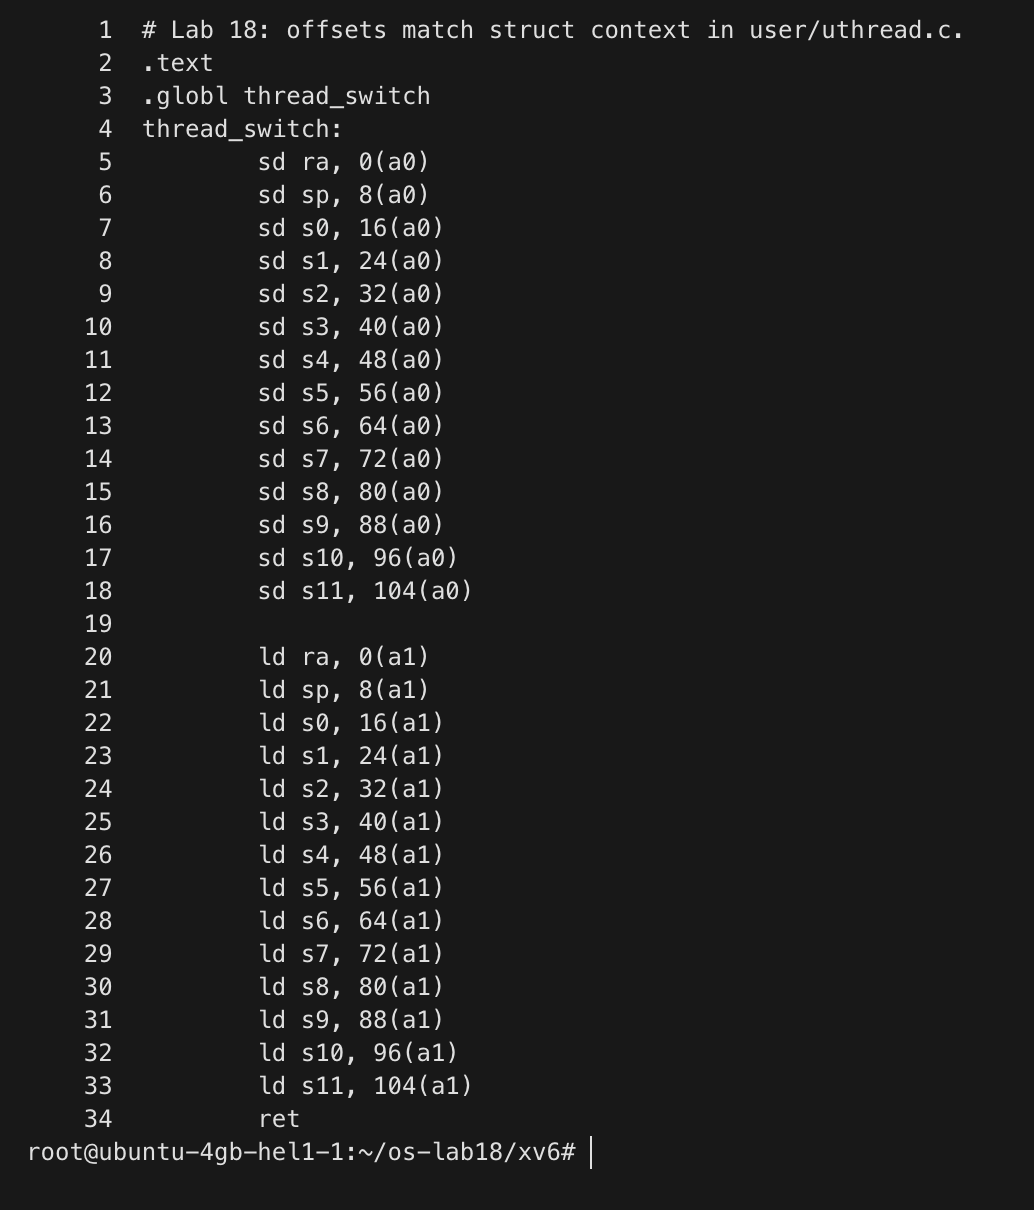
\includegraphics[width=\linewidth,height=0.67\textheight,keepaspectratio]{Lab18/evidence/screenshots/lab18-switch-assembly-terminal.png}
\end{minipage}\par\medskip

The native source capture shows all fourteen stores at lines 5--18:
{\ttfamily\fontsize{10}{12}\selectfont ra},
{\ttfamily\fontsize{10}{12}\selectfont sp}, and
{\ttfamily\fontsize{10}{12}\selectfont s0–s11} are saved through the
old-context pointer in {\ttfamily\fontsize{10}{12}\selectfont a0}. Lines
20--33 restore the same registers through the next-context pointer in
{\ttfamily\fontsize{10}{12}\selectfont a1}, using identical offsets from
0 to 104 in steps of eight bytes. Line 34 executes
{\ttfamily\fontsize{10}{12}\selectfont ret}, which transfers control
through the restored {\ttfamily\fontsize{10}{12}\selectfont ra}. The
matching store/load layout agrees with the C context shown in the
previous capture. This image documents the complete source routine; the
recorded QEMU runs and native execution-final capture demonstrate its
behavior.

\subsection{Part 2 --- Actual run and
validation}\label{part-2-actual-run-and-validation}

The recorded first run begins:

\par\noindent\begin{minipage}{\linewidth}

\begin{lstlisting}
$ uthread
thread_a started
thread_b started
thread_c started
thread_c 0
thread_a 0
thread_b 0
thread_c 1
thread_a 1
thread_b 1
\end{lstlisting}

\end{minipage}\par

After all 300 counter lines, its final round and termination are:

\par\noindent\begin{minipage}{\linewidth}

\begin{lstlisting}
thread_c 99
thread_a 99
thread_b 99
thread_c: exit after 100
thread_a: exit after 100
thread_b: exit after 100
thread_schedule: no runnable threads
\end{lstlisting}

\end{minipage}\par

These are the actual beginning and end excerpts; the omitted middle is
retained in full in the execution log. A and B yield while waiting for
the other started flags. C sets the last flag, so C prints the first
count, followed by A and B. Repeated voluntary yields preserve this
round-robin pattern.

{\ttfamily\fontsize{10}{12}\selectfont check-lab18.\allowbreak{}py}
verified ten complete runs: each had exactly three start lines, 300
count lines in {\ttfamily\fontsize{10}{12}\selectfont c,a,b} rounds from
0 through 99, three exit-after-100 lines and one final scheduler
diagnostic. Each run therefore had 307 output lines. Every run matched
the entire expected sequence, rather than merely containing a success
substring. All ten passed. A subsequent
{\ttfamily\fontsize{10}{12}\selectfont trace 32 grep hello README} still
logged the read system calls, checking the retained Lab 10
functionality.

The final diagnostic is the handout's expected no-runnable case. The
process calls {\ttfamily\fontsize{10}{12}\selectfont exit(-1)} there
after the three workers have finished; the checker requires their
complete output before accepting this terminal condition. These are
cooperative user threads, not three independently runnable kernel
threads. Even with QEMU CPUS=3, one xv6 process executes one of these
user contexts at a time.

\subsection{Native Terminal evidence --- startup and first
round}\label{native-terminal-evidence-startup-and-first-round}

\par\medskip\noindent\begin{minipage}{\linewidth}\setstretch{1.0}
\captionof*{figure}{Figura 3. Native xv6 Terminal: boot, uthread command, three started messages and the first c–a–b round}
\centering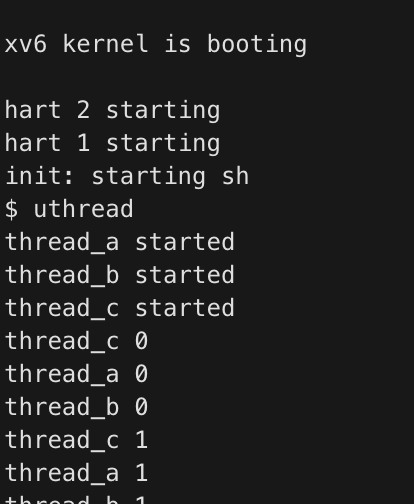
\includegraphics[width=\linewidth,height=0.67\textheight,keepaspectratio]{Lab18/evidence/screenshots/lab18-execution-start-terminal.png}
\end{minipage}\par\medskip

The supplied capture shows xv6 booting, both additional harts starting,
the shell launching, and the command
{\ttfamily\fontsize{10}{12}\selectfont uthread}. The workers announce
startup in the order A, B, C. The complete first counting round is
{\ttfamily\fontsize{10}{12}\selectfont thread\_c 0},
{\ttfamily\fontsize{10}{12}\selectfont thread\_a 0},
{\ttfamily\fontsize{10}{12}\selectfont thread\_b 0}, followed by visible
{\ttfamily\fontsize{10}{12}\selectfont thread\_c 1} and
{\ttfamily\fontsize{10}{12}\selectfont thread\_a 1}. The next line is
cut by the bottom of the supplied image, so it is not used as evidence
of a complete second round. The full execution logs retain all rounds,
while the final native capture below shows the last rounds and
termination.

This startup agrees with the flag-wait logic: A and B yield until the
other workers have started; C sets the last flag and begins counting
first. The boot messages demonstrate the three-hart QEMU environment,
but these user contexts still execute cooperatively inside a single xv6
process.

\subsection{Native Terminal evidence --- final rounds and
termination}\label{native-terminal-evidence-final-rounds-and-termination}

\par\medskip\noindent\begin{minipage}{\linewidth}\setstretch{1.0}
\captionof*{figure}{Figura 4. Native xv6 Terminal: final c–a–b rounds through 99, three exit-after-100 messages and scheduler termination}
\centering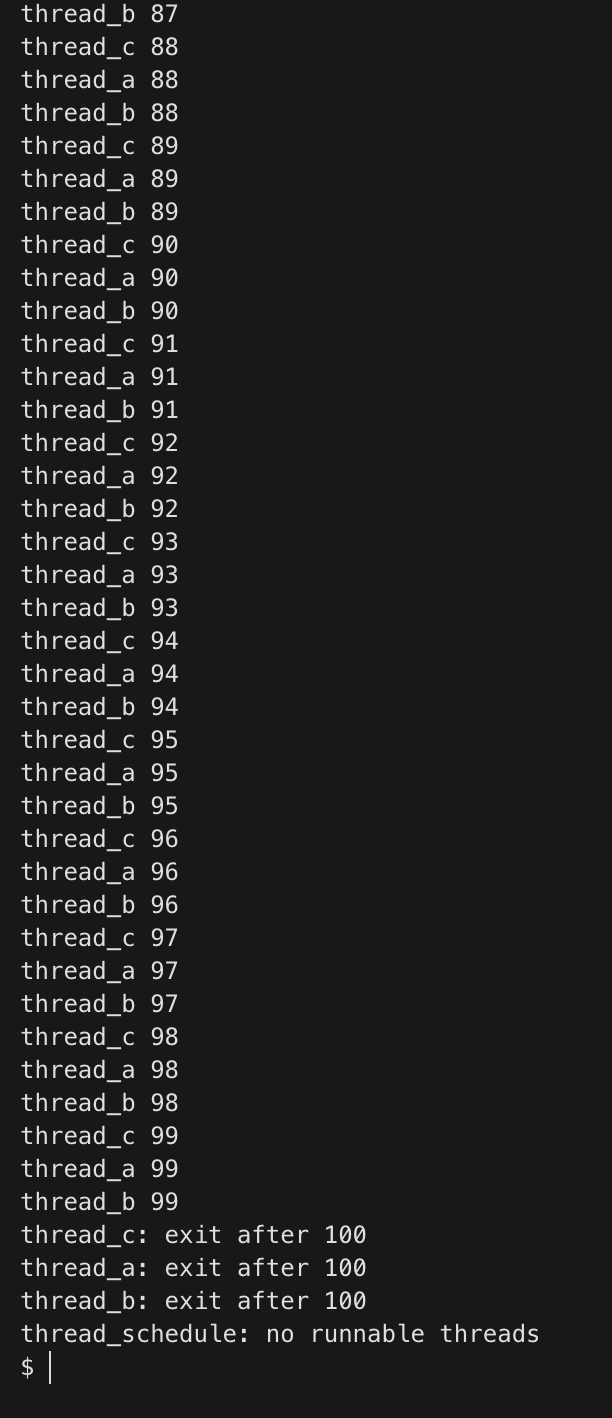
\includegraphics[width=\linewidth,height=0.67\textheight,keepaspectratio]{Lab18/evidence/screenshots/lab18-execution-finish-terminal.png}
\end{minipage}\par\medskip

The supplied execution capture begins with
{\ttfamily\fontsize{10}{12}\selectfont thread\_b 87} and then shows
every round from 88 through 99 in the order
{\ttfamily\fontsize{10}{12}\selectfont thread\_c},
{\ttfamily\fontsize{10}{12}\selectfont thread\_a},
{\ttfamily\fontsize{10}{12}\selectfont thread\_b}. The three workers
each report {\ttfamily\fontsize{10}{12}\selectfont exit after 100},
followed by
{\ttfamily\fontsize{10}{12}\selectfont thread\_sched\allowbreak{}ule: no runnable threads}
and the shell prompt. This confirms the displayed final alternation and
completion of all three workers. The initial
{\ttfamily\fontsize{10}{12}\selectfont started} messages and early
rounds are outside this image; the full automated executions remain
available in the raw log, and the separate native startup capture above
documents that part visually.

The scheduler diagnostic is the expected terminal path of the supplied
skeleton after all worker slots become FREE. Together with the three
completion messages, it indicates that the scheduler exhausted its
runnable work, rather than demonstrating a failed context switch.

\subsection{Observe --- What is saved, and why does ra transfer
control?}\label{observe-what-is-saved-and-why-does-ra-transfer-control}

The switch saves and restores
{\ttfamily\fontsize{10}{12}\selectfont ra},
{\ttfamily\fontsize{10}{12}\selectfont sp}, and all twelve
{\ttfamily\fontsize{10}{12}\selectfont s} registers at offsets 0 through
104. Under the calling convention the caller already treats argument and
temporary registers as call-clobbered, while the
{\ttfamily\fontsize{10}{12}\selectfont s} registers must survive a call.
The saved stack pointer restores the other worker's call frames and
local variables. This exercise uses integer contexts and does not
implement floating-point thread state.

The call to
{\ttfamily\fontsize{10}{12}\selectfont thread\_switc\allowbreak{}h}
places its continuation address in
{\ttfamily\fontsize{10}{12}\selectfont ra}. When that context is
restored, {\ttfamily\fontsize{10}{12}\selectfont ret} resumes the
suspended scheduler call in that worker. For a newly created thread, the
initial {\ttfamily\fontsize{10}{12}\selectfont ra} instead names its
entry function. Loading the other context's
{\ttfamily\fontsize{10}{12}\selectfont ra} and executing
{\ttfamily\fontsize{10}{12}\selectfont ret} therefore transfers
execution to that context; there is no separate saved program-counter
field in this cooperative call/return design. The same explanation is
supplied in the required
{\ttfamily\fontsize{10}{12}\selectfont notes.txt}.

\subsection{Reproduction and captures}\label{reproduction-and-captures}

Build from {\ttfamily\fontsize{10}{12}\selectfont xv6/} with
{\ttfamily\fontsize{10}{12}\selectfont make kernel/kerne\allowbreak{}l fs.img},
then run {\ttfamily\fontsize{10}{12}\selectfont make qemu CPUS=3} and
enter {\ttfamily\fontsize{10}{12}\selectfont uthread} at the xv6 prompt.
To rerun the automated checks from the repository root, use
{\ttfamily\fontsize{10}{12}\selectfont python3 Lab18/check-\allowbreak{}lab18.py xv6 /tmp/os-lab1\allowbreak{}8-evidence}.
It boots the existing built image and writes real output to the selected
directory. Keep a separate generated filesystem image if it contains
files you wish to preserve. The screenshot plan covers context
initialization, assembly, startup/first rounds and final
counts/termination.

\par\noindent\begin{minipage}{\linewidth}

\section{Concluzie}\label{concluzie}

Cele zece execuții verificate au păstrat ordinea c--a--b și câte 100 de
iterații pentru fiecare fir. Contextul și stivele separate permit
reluarea corectă a apelurilor suspendate, fără modificări în kernel.
Cele patru capturi native documentează contextul, rutina assembly,
începutul și finalul execuției, completând jurnalul integral.

\end{minipage}\par

\end{document}
